\section{Erweiterung der Eingabe}
\label{sec:sha256:erweiterung}

Um für jede der 64 Runden einen 32 Bit Eingabewert berücksichtigen zu können, wird die Eingabe von 512 Bit auf 2048 Bit erweitert.
Dabei kommen sowohl die modulare 32-Bit Addition als auch die beiden $\sigma$-Funktionen zum Einsatz.
Für die ersten 16 Runden wird die Eingabe direkt übernommen. Für alle weiteren Runden werden vier vorhergehende Eingaben zur Berechnung
gemäß Abbildung \ref{fig:sha256prep} herangezogen. Das führt dazu, dass die Eingabe einer Runde nicht nur bis zu vier nachfolgenden
Runden beeinflusst, sondern auch Auswirkungen auf weitere Runden hat, weil diese wiederum in nachfolgenden Runden verwendet wird.

\begin{figure}[!h]
  \centering
  \begin{minipage}[c]{5cm}
    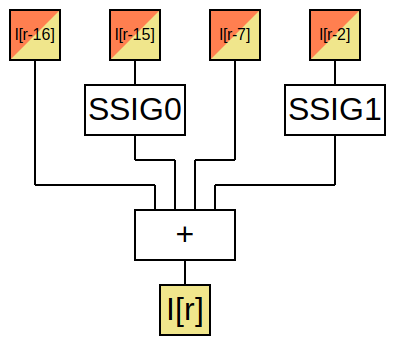
\includegraphics[scale=0.4]{images/sha256prepS}
  \end{minipage}
  \begin{minipage}[c]{6cm}
    \begin{align}
      I[r] = \sigma_1(I[r-2]) + I[r-7] + \sigma_0(I[r-15]) + I[r-16] \nonumber
    \end{align}
  \end{minipage}
  \caption{Schematische Darstellung der Erweiterung}
  \label{fig:sha256prep}
\end{figure}